\chapter{Representation Predicates}
\label{predicates}

\epigraph{One might say, by way of excuse, ``but the language in which I program has the kind of address arithmetic that makes it impossible to know the bounds of an array." Yes, and the man who shot\\his mother and father threw himself upon the mercy of the court because he was an orphan.}{Andrew W. Appel~\cite{appel1998modern}}
% page 160 in ML, page 168 in Java. Chapter 7.2

In code compiled from Coq to C by CertiCoq, Coq values are uniformly represented in memory. Foreign C functions called from Coq are expected to take inputs and give outputs in this representation, yet nothing stops them from flouting this expectation. A violation of this representation may cause a runtime error, but there is no way to catch it statically or prove that no such violation exists. In this chapter, I will describe the uniform memory representation of Coq values, I will introduce representation predicates, a mechanism to state the proposition that a Coq value in CertiCoq's heap memory truly represents that value and also respects this uniform representation, unless it is a value of a \gls{foreign type} with a custom representation. I will also describe the automatic generation of representation predicates. 
% And on the other hand, user-defined \gls{foreign type}s (implemented in C) need not have uniform representations, yet they must also fit into this specification framework, as I will explain.\todo{TODO: Did I explain?}

\section{Memory Representation of Values}
\label{memoryrepresentation}

CertiCoq's memory representation of values is almost identical to OCaml's memory representation of values~\cite{madhavapeddy2022real}. This similarity is no coincidence; it was a design choice that is meant to provide compatibility with OCaml programs, to have the option to use code written for OCaml's backend (such as its garbage collector)~\cite{certicoq}, and eventually maybe even to use CertiCoq to compile OCaml code.

Since the representation predicates we present in this thesis are so closely tied to the memory representation of values, let us revisit it and understand how CertiCoq represents Coq values in memory.

A Coq value is a single word (32 bits or 64 bits depending on the machine) in memory that is either an unsigned integer or a pointer to another block of words in memory. We fit all Coq values in this format.

Coq has four kinds of values: types, \constructor{}s, function \gls{closure}s, and \gls{primitive} values.

Types and values of sort \ty{Prop} are erased from CertiCoq early in the compiler pipeline~\cite{certicoq, belanger2019verified, paraskevopoulou2020verified}. Any function that takes a type argument or a \ty{Prop} value in Coq still takes that argument in the generated C code, but the erased value is computationally irrelevant: It is never inspected and is always represented by the integer \dt{1} in CertiCoq's C runtime.

Constructors have either \emph{\gls{boxed}} or \emph{\gls{unboxed}} representation.
Constructors that take arguments have \gls{boxed} representation; they are represented by a pointer that points to a block of words:

\begin{figure}[H]
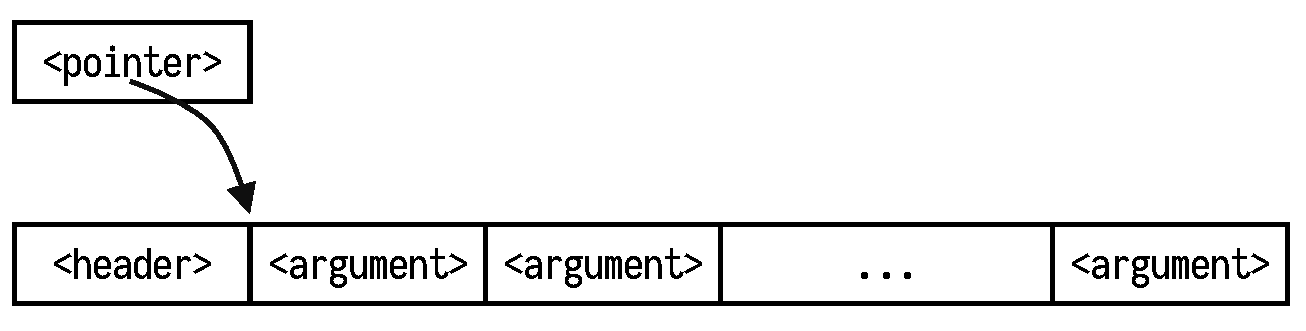
\includegraphics[scale=.59]{figures/boxed-value.pdf}
\centering
\caption{A \gls{boxed} representation of a \constructor{}.}
\end{figure}

\newpage
A \gls{boxed} value has a pointer address, which points to the second word of a block in memory where there is a \header{} and the arguments of the \constructor. 

Here is what the \header{} for a \gls{boxed} \constructor{} looks like when the word size is 64:

\begin{figure}[H]
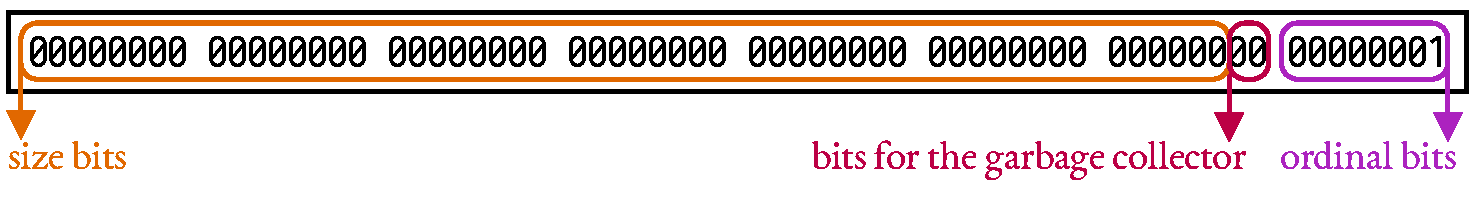
\includegraphics[scale=.59]{figures/boxed-header.pdf}
\centering
\caption{The header of a \gls{boxed} \constructor{}.}
\end{figure}

The first 22 or 54 bits (depending on the word size of the machine) of the \header{} signify the size of the block (in words) that comes after the \header{}. For a \gls{boxed} inductive Coq \constructor, this essentially means the number of arguments.\footnote{For types that have \glspl{parameter} or \glslink{index}{indices}, keep in mind that the parameter will not exist in runtime, but the index always will.}

Constructors that take no arguments have \gls{unboxed} representation, so there is no header, and no block, and no pointer: instead there is an odd number.

Here is what an unboxed constructor looks like when the word size is 64:

\begin{figure}[H]
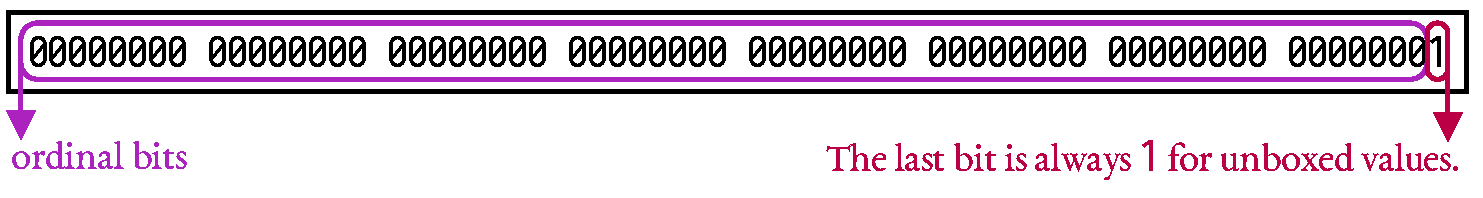
\includegraphics[scale=.59]{figures/unboxed-value.pdf}
\centering
\caption{An \gls{unboxed} representation of a \constructor{}.}
\end{figure}

Function \gls{closure}s are represented as a pointer to a block of memory, where a function pointer and its environment live. The environment is represented as a linked list in runtime. However, the environment is not typeable in Coq, as the values in the environments can be of different types.
% \todo{Higher-order, GraphPredicate of functions? call?}

\Gls{primitive} values have their own custom representations, which we will examine later in this thesis.

\subsection{Representation in the Heap Graph}

Based on the description above of CertiCoq's memory representation of values, one might assume that each Coq value has its own memory block. From a graph theory perspective, this assumption would have made the CertiCoq heap an \emph{out-forest}. Each Coq value would then be represented in the graph as an \emph{out-tree}. This, while elegant, is unfortunately not the case. DAGs in the heap graph can occur naturally: For terms such as \code{(\bn{x}, \bn{x})} or \code{[\bn{x}; \bn{x}; \bn{x}]}, the created object would be a DAG, not an out-tree. Even for Coq values that are created as out-trees initially, garbage collection can change the graph in a way that violates the tree properties, specifically because a path in the graph would not be necessarily unique anymore. The graph we arrive at is a \emph{directed acyclic graph} (DAG) but not an out-forest. The heap graph below is an example of this change: The object on the left can turn into the object on the right when the garbage collector runs, if we are using a hash-consing garbage collector~\cite{appel1993hash}.

\begin{figure}[H]
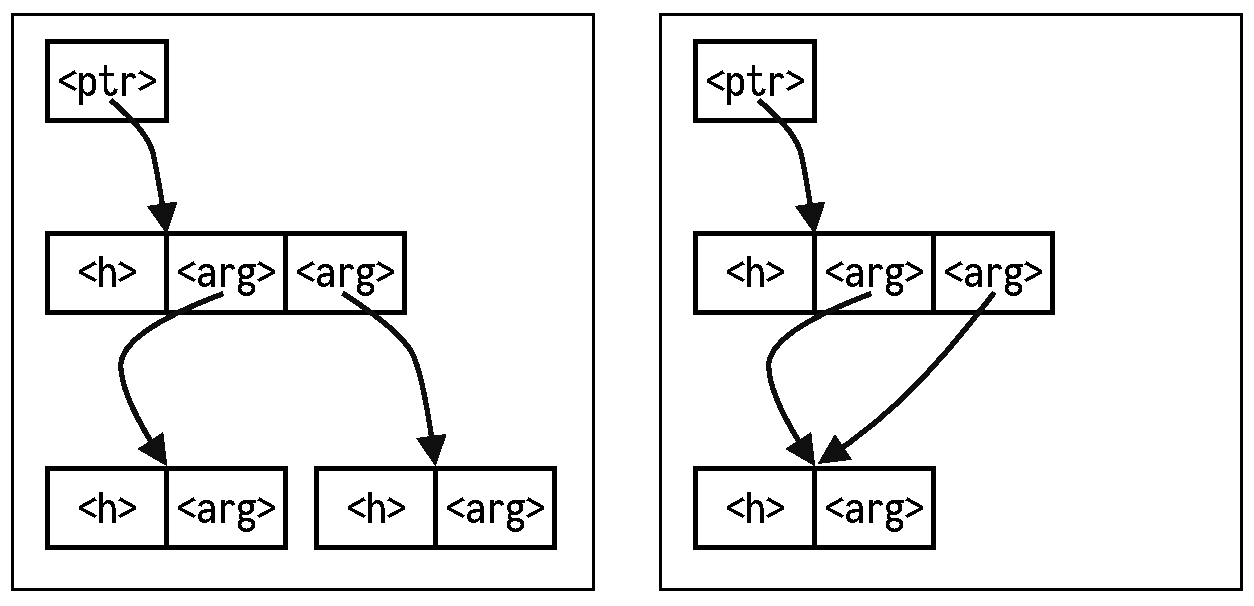
\includegraphics[scale=.49]{figures/gcdual.pdf}
\centering
\caption{Two possible memory representations of the term \code{(\dt{S O}, \dt{S O})}.}
\end{figure}

% Andrew's note:
% This is technically correct, but it is not the main reason that out-DAGs exist.   Most garbage collectors, including CertiCoq's current one, do not turn trees into DAGs.  Only the weird ones described in [Appel and Goncalves] would do that. Instead, the out-DAGs arise from ordinary interpreted or compiled Coq code, in which we can write (x,x) which creates a tuple that's already a DAG. (Or: x::x::x::nil)
% Hash-Consing Garbage Collection, by Andrew W. Appel and Marcelo J.R. Goncalves, Technical report TR-412-93, Department of Computer Science, Princeton University, January 1993.

Here on both sides, we see the term \code{(\dt{S O}, \dt{S O})}. The root of the \gls{boxed} \constructor{} for pairs. Each field of the pair is a boxed constructor for the successor constructor \dt{S}. In both of the successors, we see an \gls{unboxed} constructor \dt{O}. However, since the \dt{S O} value occurs twice, the garbage collector can free the memory used for one of them and have both values point to the same memory block so that the representation is shared between two values.

Since memory blocks are shared for different values, we cannot simply depend on the $\mathrel{*}$ connective in separation logic. At this point, we rely on previous work and use the CertiGraph library, which helps us reason about graph manipulating programs in VST~\cite{wang2019graph, shengyi2020mechanized}. The CertiGraph project developed a mechanically verified garbage collector for the CertiCoq runtime. We use both their garbage collector implementation in the CertiCoq runtime and their library of proofs to write our proofs about foreign functions.

\section{Definition of Representation Predicates}
\label{predicatedefns}

Correctness specifications of \constructor{} \glue{} functions and \gls{foreign function}s will involve (among other things) the correct interpretation and production of Coq values in the uniform representation we described above.
In this chapter, I will describe \emph{representation predicate}s, a mechanism to assert that a Coq value in CertiCoq's heap memory respects this uniform representation, and is equal to a certain Coq value. Using representation predicates, we can express specifications about the correctness and type safety of \glue{} functions and \gls{foreign function}s.


The memory representation of values is uniform, but only for values of \gls{inductive type}s and \gls{closure}s. \Gls{primitive} values and values of \gls{foreign type}s are allowed to have custom representations, therefore our system should be able to express custom representations. Therefore, we use Coq's type classes~\cite{sozeau2008first} to define graph predicates; this allows us to overload a single function name with different definitions for uniform representations of different \gls{inductive type}s, and also custom representations of \gls{foreign type}s:

\newcommand{\GraphPredicate}{\hyperref[code:GraphPredicate]{\ty{GraphPredicate}}}
\newcommand{\graphpredicate}{\hyperref[code:graphpredicate]{\fn{graph\_\linebreak[0]predicate}}}
\begin{Verbatim}
\kw{Class} \label{code:GraphPredicate}\GraphPredicate (\bn{A} : \ty{Type}) : \ty{Type} :=
  \{ \label{code:graphpredicate}\graphpredicate : \ty{graph} -> \ty{outlier_t} -> \bn{A} -> \ty{rep_type} -> \ty{Prop} \}.
\end{Verbatim}


We define a graph predicate as a function that takes the heap graph, the outliers (i.e.\ the values that are used but live outside of the \gls{CertiCoq heap}), an actual Coq value, and a heap representation, and produces a \ty{Prop} that posits that the heap representation represents the given Coq value in the heap graph properly.

For most types, we generate and use the common instance that follows the uniform representation. However, the type class mechanism allows the user to write custom instances of the \GraphPredicate{} type class, where the user can specify the layout of values of a particular type in the heap graph. As examples for custom representations, we will implement our own \gls{primitive} integers in \autoref{integers}, and our own \gls{primitive} strings in \autoref{bytestrings}.

During our proofs, we will need some lemmas about our graph predicate function. These lemmas are automatically proven for the uniform representation of inductive types, while the user will have to prove them by hand for custom representations. Because of the intricacy of their generation (explained further in \autoref{predicategen}), these lemmas live in a separate type class:

\newcommand{\InGraph}{\hyperref[code:InGraph]{\ty{InGraph}}}
\newcommand{\ingraphpred}{\hyperref[code:ingraphpred]{\fn{in\_\linebreak[0]graph\_\linebreak[0]pred}}}
\newcommand{\hasv}{\hyperref[code:hasv]{\fn{has\_v}}}
\newcommand{\ismonotone}{\hyperref[code:ismonotone]{\fn{is\_\linebreak[0]monotone}}}
\newcommand{\outliercompat}{\hyperref[code:outliercompat]{\fn{outlier\_\linebreak[0]compat}}}
\label{code:InGraph}
\label{code:ingraphpred}
\label{code:ismonotone}
\label{code:outliercompat}
\begin{Verbatim}
\kw{Class} \InGraph (\bn{A} : \ty{Type}) : \ty{Type} :=
  \{ \ingraphpred{} : \GraphPredicate \bn{A}
  ; \label{code:hasv}\hasv :
      \kw{forall} (\bn{g} : \ty{graph}) (\bn{outliers} : \ty{outlier_t}) (\bn{n} : \bn{A}) (\bn{v} : \ty{VType}),
        \graphpredicate \bn{g} \bn{outliers} \bn{n} (\fn{repNode} \bn{v}) -> \fn{graph_has_v} \bn{g} \bn{v}
  ; \ismonotone{} :
      \kw{forall} (\bn{g} : \ty{graph}) (\bn{outliers} : \ty{outlier_t}) (\bn{to} : \ty{nat}) (\bn{lb} : \ty{raw_vertex_block})
             (\bn{e} : \ty{list edge}) (\bn{n} : \bn{A}) (\bn{p} : \ty{rep_type}),
        \fn{add_node_compatible} \bn{g} (\fn{new_copied_v} \bn{g} \bn{to}) \bn{e} ->
        \fn{graph_has_gen} \bn{g} \bn{to} -> 
        \graphpredicate \bn{g} \bn{outliers} \bn{n} \bn{p} -> 
        \graphpredicate (\fn{add_node} \bn{g} \bn{to} \bn{lb} \bn{e}) \bn{outliers} \bn{n} \bn{p}
  ; \outliercompat{} : 
      \kw{forall} (\bn{g} : \ty{graph}) (\bn{outliers} : \ty{outlier_t}) (\bn{x} : \bn{A}) (\bn{p} : \ty{GC_Pointer}),
        \fn{outlier_compatible} \bn{g} \bn{outliers} ->
        \graphpredicate{} \bn{g} \bn{outliers} \bn{x} (\dt{repOut} \bn{p}) ->
        \ty{In} \bn{p} \bn{outliers}
  \}.
\end{Verbatim}

This type class contains
\begin{itemize}
\item the \GraphPredicate{} instance,
\item the \hasv{} lemma, which states that if a value is represented in the graph as a node, then the vertex of the node is in the graph,
\item the \ismonotone{} lemma, which states that a Coq value that is represented in memory properly can still be represented in memory if a new compatible node is added to the heap graph,
\item and the \outliercompat{} lemma, which states that if a Coq value is represented in the \gls{C heap} (as an \emph{outlier}), then that pointer will be in the outlier set.
\end{itemize}
The components of this type class are the work of Stark and Appel. This thesis does not require a deep understanding of these components because this thesis is mostly about writing foreign functions and their specifications, and not so much the proofs of these specifications. Therefore we will not go further in detail here, but the details of these lemmas can lemmas can be found in the tech report by Korkut, Stark, and Appel~\cite{korkutStarkAppel}.

Since we now have a type class hierarchy of \GraphPredicate{} and \InGraph{}, we also define the following helper function that projects the \graphpredicate{} field of the superclass \GraphPredicate{}, from an instance of the subclass \InGraph{}:

\newcommand{\isingraph}{\hyperref[code:isingraph]{\fn{is\_\linebreak[0]in\_\linebreak[0]graph}}}
\label{code:isingraph}
\begin{Verbatim}
\kw{Definition} \isingraph{} \{\bn{A} : \ty{Type}\} `\{\InGraph \bn{A}\}
                       : \ty{graph} -> \ty{outlier_t} -> \bn{A} -> \ty{rep_type} -> \ty{Prop} :=
  @\graphpredicate \bn{A} \ingraphpred.
\end{Verbatim}


Using these predicates, the users are empowered to write their own specifications and proofs for their foreign C functions. These predicates are also used to generate specifications and proofs for CertiCoq-generated glue functions, which can be used as building blocks for the foreign C functions and their correctness proofs.

For example, the \GraphPredicate{} instance for the \Vec{} inductive type looks like this:

% \newpage
\label{code:GraphPredicatevec}
\newcommand{\GraphPredicatevec}{\hyperref[code:GraphPredicatevec]{\fn{GraphPredicate\_\linebreak[0]vec}}}
\begin{Verbatim}
\kw{Instance} \GraphPredicatevec
         (\bn{A} : \ty{Type}) 
         (\bn{GraphPredicate_A} : \GraphPredicate{} \bn{A})
         (\bn{n} : \ty{nat}) : \GraphPredicate{} (\ty{vec} \bn{A} \bn{n}) :=
  \kw{let} \kw{fix} \fn{graph_predicate_vec} 
          (\bn{n} : \ty{nat})
          (\bn{g} : \ty{graph}) (\bn{outliers} : \ty{outlier_t}) (\bn{x} : \ty{vec} \bn{A} \bn{n}) (\bn{p} : \ty{rep_type})
          \{\kw{struct} \bn{x}\} : \ty{Prop} :=
    \kw{match} \bn{x} \kw{with}
    | \dt{vnil} => \fn{graph_cRep} \bn{g} \bn{p} (\dt{enum} \dt{0}) \dt{[]}
    | \dt{vcons} \bn{arg0} \bn{arg1} \bn{arg2} =>
        \kw{exists} \bn{p0} \bn{p1} \bn{p2} : \ty{rep_type},
          @\graphpredicate{} \ty{nat} \fn{GraphPredicate_nat} \bn{g} \bn{outliers} \bn{arg0} \bn{p0} \ty{/\textbackslash}
          @\graphpredicate{} \bn{A} \bn{GraphPredicate_A} \bn{g} \bn{outliers} \bn{arg1} \bn{p1} \ty{/\textbackslash}
          \fn{graph_predicate_vec} \bn{arg0} \bn{g} \bn{outliers} \bn{arg2} \bn{p2} \ty{/\textbackslash}
          \fn{graph_cRep} \bn{g} \bn{p} (\dt{boxed} \dt{0} \dt{3}) \dt{[}\bn{p0}\dt{;} \bn{p1}\dt{;} \bn{p2}\dt{]}
    \kw{end}
  \kw{in} \{| \graphpredicate{} := (\fn{graph_predicate_vec} \bn{n}) |\}.
\end{Verbatim}


\section{Generation of Representation Predicates}
\label{predicategen}

We generate for the \GraphPredicate{} and the \InGraph{} type classes using MetaCoq.

The \GraphPredicate{} type class only contains one field, the predicate function, and is generated entirely with MetaCoq. We made this design choice because the generated term has many moving parts: The instance has to quantify over the \gls{parameter}s and \indices{} of the inductive type. If those parameters are types, then the instance has to quantify over the \GraphPredicate{} instance of them. Parameters stay the same for the types in the same mutually inductive block, while indices can vary, which means the \kw{fix} we generate has to quantify over the indices. The \GraphPredicatevec{} example above demonstrates all of these moving parts.

Instances of the \InGraph{} type class, on the other hand, are generated using a combination of MetaCoq and \gls{Ltac}. We use MetaCoq only for generating the types of the instances and invoking \gls{Ltac} using \tmLemma{}. While these instances still have quantified \gls{parameter}s and \indices{}, the definitions inside an \InGraph{} instance do not need to use a \kw{fix} expression, so they are easier to discharge with \gls{Ltac} than to build with MetaCoq.

In this section, we will examine the problems we encounter with generating instances for the \GraphPredicate{} and \InGraph{} type classes, and present techniques to solve these problems.

\subsection{De Bruijn Notation Conversion}
\label{debruijnconversion}

In MetaCoq, variables are represented using a \emph{\gls{locally nameless}}~\cite{aydemir2008} approach\footnote{There is one caveat: While it is common to remove names from quantifiers in a \gls{locally nameless} representation, MetaCoq retains them.}. This means that free variables are represented as names, while bound variables are represented as de Bruijn indices~\cite{de1972lambda}. The \ty{term} type in MetaCoq, which deeply embeds the core terms of \gls{Gallina}, includes 4 constructors that are relevant to variables.

\begin{Verbatim}
\kw{Inductive} \ty{term} : \ty{Type} :=
    \dt{tRel} : \ty{nat} -> \ty{term}
  | \dt{tVar} : \ty{ident} -> \ty{term}
  | \dt{tEvar} : \ty{nat} -> \ty{list term} -> \ty{term}
  | \dt{tConst} : \ty{kername} -> \ty{Instance.t} -> \ty{term}
  ...
\end{Verbatim}

\dt{tRel} represents variables referred to by a de Bruijn index, where the lowest number in \dt{tRel} refers to the latest variable binding.
\dt{tVar} represents named variables introduced in Coq sections or interactive proofs~\cite{sozeau2020metacoq}. However, we will use \dt{tVar} for more than that soon.
\dt{tEvar} represents existential variables, which do not have locally nameless representation except in their sub\ty{term}s.
\dt{tConst} represents constants (but not inductive types or constructors), i.e. free variables that have a fully qualified name.

Let us consider an example of a quoted term that can help illustrate:

\vspace{.2in}
\begin{SaveVerbatim}{E}
\kw{MetaCoq Run} (\fn{tmQuote} (\kw{fun} (\bn{A} : \ty{Type}) (\bn{a} : \bn{A}) => \bn{a}) \fn{>>}\fn{=} \fn{tmPrint}).
\end{SaveVerbatim}
\tocoq{\UseVerbatim{E}}

\begin{SaveVerbatim}{E}
\dt{tLambda} \{| \fn{binder_name} := \dt{nNamed "A"}; \fn{binder_relevance} := \dt{Relevant} |\}
   (\dt{tSort} ...)
   (\dt{tLambda} \{| \fn{binder_name} := \dt{nNamed "a"}; \fn{binder_relevance} := \dt{Relevant} |\}
            (\dt{tRel 0})
            (\dt{tRel 0}))
\end{SaveVerbatim}
\fromcoq{\UseVerbatim{E}}

Here we are quoting the polymorphic identity function, which takes one argument \bn{A} that is a type, and one more argument \bn{a} of the type \bn{A}. However, notice that in the result of the quotation, the lambda body does not mention the type \bn{A} by name; it is represented by a de Bruijn index, represented by \dt{tRel 0}. This is observable in the second argument of the inner \dt{tLambda}.
The third argument of the inner \dt{tLambda} construction represents the function body in the original lambda, also happens to be \dt{tRel 0}. The new zeroth de Bruijn index refers to the argument \bn{a}, since the latest quantifier is \bn{a} now.

As we can see from this term, having quoted terms in de Bruijn notation can be confusing when inspecting quoted terms; it is even more confusing and error-prone to generate terms to unquote. This is because the code we want to generate will often have to deal with varying numbers of \indices{} or \gls{parameter}s of \gls{inductive type}s. Committing to generating code in de Bruijn notation will mean we have to keep track of how many of these \indices{} and \gls{parameter}s we have at a given time. Considering the possibility of our generated code introducing new quantifiers and having complicated dependent types that themselves can contain de Bruijn indices, it becomes clear that this is unsustainable.

Our solution is to misuse the \dt{tVar} constructor creatively to have a named representation for our terms. In this representation, all bound variables will be represented as \dt{tVar}s instead of \dt{tRel}s. We can define a function that converts between named and locally nameless representations. Any \ty{term} we receive from \TemplateMonad{} \gls{primitive}s or we pass into \TemplateMonad{} \gls{primitive}s will have locally nameless representation. But for the remaining internal computation, we can use our named representation.

\begin{Verbatim}
\kw{Definition} \ty{named_term} : \ty{Type} := \ty{term}.

\kw{Definition} \fn{deBruijn} (\bn{ctx} : \ty{list name}) (\bn{t} : \ty{named_term}) : \TemplateMonad{} \ty{term} :=
  ...
\kw{Definition} \fn{closed_deBruijn} (\bn{t} : \ty{named_term}) : \TemplateMonad{} \ty{term} :=
  \fn{deBruijn} \dt{nil} \bn{t}.

\kw{Definition} \fn{undeBruijn} (\bn{ctx} : \ty{list name})  (\bn{t} : \ty{term}) : \TemplateMonad{} \ty{named_term} :=
  ...
\kw{Definition} \fn{closed_undeBruijn} (\bn{t} : \ty{term}) : \TemplateMonad{} \ty{named_term} :=
  \fn{undeBruijn} \dt{nil} \bn{t}.
\end{Verbatim}

The \fn{deBruijn} and \fn{undeBruijn} implementations are quite straightforward. They adhere to the de Bruijn notation conversion definitions commonly found in programming language textbooks. We only needed to consider the dependent type system of the \gls{Gallina} core language and the fact that pattern matching in \kw{match} expressions can alter the number of bindings in the branch body.

\subsection{Type Class Resolution}

MetaCoq does not provide a mechanism for type class resolution under a context. We need to find a way to make unquotable \ty{term}s quotable (as we will explain) in order to use the \gls{primitive} resolution mechanism. Our solution for this problem is lambda lifting~\cite{johnsson1985lambda}. 

As seen in the \GraphPredicatevec{} instance above, we need to call \graphpredicate{} for the argument types of constructors. Given that \graphpredicate{} is a method of the \GraphPredicate{} type class, we have to make sure MetaCoq can figure out the type class instance to be used in the call. The initial solution most MetaCoq users would go for is to leave the instance argument as a \fn{hole}, and for MetaCoq to figure out how to fill the \fn{hole} during \gls{unquotation}. Unfortunately, this solution is currently not reliable enough, therefore we will have to infer these type class instances manually. MetaCoq only provides the following mechanism for type class resolution:

\vspace{.2in}
\begin{SaveVerbatim}{E}
\kw{Check} \fn{tmInferInstance}.
\end{SaveVerbatim}
\tocoq{\UseVerbatim{E}}

\begin{SaveVerbatim}{E}
\fn{tmInferInstance}
     : \ty{option reductionStrategy} -> 
       \kw{forall} \bn{A} : \ty{Type}, \TemplateMonad{} (\ty{option_instance} \bn{A})
\end{SaveVerbatim}
\fromcoq{\UseVerbatim{E}}

\newpage
Observe that this \TemplateMonad{} \gls{primitive} takes a \ty{Type}, and not a \ty{term}. This is easy to call with an actual type class constraint:

\vspace{.2in}
\begin{SaveVerbatim}{E}
\kw{MetaCoq Run} (\fn{tmInferInstance} (\dt{Some all}) 
                             (\kw{forall} \bn{A} `\{\ty{GraphPredicate} \bn{A}\} \bn{n},
                              \ty{GraphPredicate} (\ty{vec} \bn{A} \bn{n}))
             \fn{>>}\fn{=} \fn{tmPrint}).
\end{SaveVerbatim}
\tocoq{\UseVerbatim{E}}

\begin{SaveVerbatim}{E}
(\dt{my_Some} _ \fn{GraphPredicate_vec})
\end{SaveVerbatim}
\fromcoq{\UseVerbatim{E}}

However, when we inspect an \gls{inductive type}, we usually work with the reified versions of types and constructors. In order to use the \fn{tmInferInstance} \gls{primitive}, we would have to \unquote{} the \ty{term} into the Coq value it represents. Unfortunately, \unquoting{} can sometimes fail. Many intermediate forms we obtain while we compute results with \ty{term}s are not suitable to \unquoting{}. Consider the following function, one we actually use in the generation of \GraphPredicate{} instances:

\begin{Verbatim}
\kw{Fixpoint} \fn{strip_pis} (\bn{t} : \ty{named_term}) : \ty{named_term} :=
  \kw{match} \bn{t} \kw{with}
  | \dt{tProd} _ _ \bn{rest} => \fn{strip_pis} \bn{rest}
  | \bn{x} => \bn{x}
  \kw{end}.
\end{Verbatim}

This function takes a full function or constructor type, and removes the surrounding function type binders ($\Pi$-types, hence the function name). If it is given a term representing \code{\kw{forall} (\bn{A} : \ty{Type}), \bn{A}}, it will return a term that represents \bn{A}, i.e. the result type of the original function type.

This function generates unquotable terms for two reasons. One reason is that the stripped result type will contain free variables, therefore \unquoting{} will fail. The other reason is that this function generates \ty{named\_term}s, where we have a named representation instead of a de Bruijn notation, as described in \autoref{debruijnconversion}.
The former problem is handled by lambda lifting~\cite{johnsson1985lambda}, and the latter problem is handled by de Bruijn notation conversion. 

When we are generating the branches of the \kw{match} expression, we want to be able to call \graphpredicate{} on the arguments of constructors. However, we have to keep in mind that we are dealing with reified terms representing dependently typed arguments, in named representation. We will not be able to ask MetaCoq for an instance of \code{\GraphPredicate{} (\Vec{} \bn{A} \bn{n})} because since \bn{A} and \bn{n} are free variables, this type class is not even unquotable. To make it quotable, we have to turn it into a closed term by quantifying over the free variables, which we keep as the context, and convert it to de Bruijn notation. Then we can call the \fn{tmInferInstance} \gls{primitive}, as seen in the interaction above, and obtain the relevant \GraphPredicate{} instance. However, the call to \graphpredicate{} cannot solely pass \GraphPredicatevec{} as the instance, since the instance quantifies over the free variables even though the \graphpredicate{} call does not. Therefore we have apply the context to the instance object:

\vspace{.2in}
\begin{SaveVerbatim}{E}
\kw{Variable} (\bn{A} : \ty{Type})
         (\bn{GraphPredicate_A} : \GraphPredicate{} \bn{A})
         (\bn{n} : \ty{nat}).
\kw{Check} @\graphpredicate{} (\Vec{} \bn{A} \bn{n}) (\fn{GraphPredicate_vec} \bn{A} \bn{GraphPredicate_A} \bn{n}).
\end{SaveVerbatim}
\tocoq{\UseVerbatim{E}}

\begin{SaveVerbatim}{E}
\graphpredicate{}
     : \ty{graph} -> \ty{outlier_t} -> \ty{vec} \bn{A} \bn{n} -> \ty{rep_type} -> \ty{Prop}
\end{SaveVerbatim}
\fromcoq{\UseVerbatim{E}}

As seen in the arguments passed to \GraphPredicatevec{} here, applying the context makes the instance object type check.

\newpage
\subsection{Mutually Recursive Type Class Instances}

Coq allows definitions of mutually inductive data types:

\begin{Verbatim}
\kw{Inductive} \ty{tree} (\bn{A} : \ty{Type}) : \ty{Type} :=
| \dt{tleaf} : \ty{tree} \bn{A}
| \dt{tnode} : \bn{A} -> \ty{forest} \bn{A} -> \ty{tree} \bn{A}
\kw{with} \ty{forest} (\bn{A} : \ty{Type}) : \ty{Type} :=
| \dt{fnil} : \ty{forest} \bn{A}
| \dt{fcons} : \ty{tree} \bn{A} -> \ty{forest} \bn{A} -> \ty{forest} \bn{A}.
\end{Verbatim}

Coq allows definitions of mutually recursive functions as well:

\begin{Verbatim}
\kw{Fixpoint} \fn{tree_size} \{\bn{A} : \ty{Type}\} (\bn{t} : \ty{tree} \bn{A}) : \ty{nat} :=
  \kw{match} \bn{t} \bn{with}
  | \dt{tleaf} => \dt{0}
  | \dt{tnode} _ \bn{f} => \dt{1} \fn{+} \fn{forest_size} \bn{f}
  \kw{end}
\kw{with} \fn{forest_size} \{\bn{A} : \ty{Type}\} (\bn{f} : \ty{forest} \bn{A}) : \ty{nat} :=
  \kw{match} \bn{f} \kw{with}
  | \dt{fnil} => \dt{0}
  | \dt{fcons} \bn{t} \bn{f} => \fn{tree_size} \bn{t} + \fn{forest_size} \bn{f}
  \kw{end}.
\end{Verbatim}

Notice that \kw{Fixpoint} is a vernacular command that can create multiple, mutually recursive definitions. 

However, MetaCoq does not provide a \TemplateMonad{} \gls{primitive} to create multiple definitions together. It only allows making a \gls{Gallina} term into a single definition. In \gls{Gallina} you cannot define both definitions at once, you have to define each function separately. \gls{Gallina}'s syntax for mutually recursive functions allows locally defining all functions but then exporting a single one of them at the end (with \kw{for} followed by an identifier). Here is what these two functions would look like as stand-alone definitions:

\begin{Verbatim}
\kw{Definition} \fn{tree_size} :=
  \kw{fix} \fn{tree_size} \{\bn{A} : \ty{Type}\} (\bn{t} : \ty{tree} \bn{A}) : \ty{nat} :=
    \kw{match} \bn{t} \bn{with}
    | \dt{tleaf} => \dt{0}
    | \dt{tnode} _ \bn{f} => \dt{1} \fn{+} \fn{forest_size} \bn{f}
    \kw{end}
  \kw{with} \fn{forest_size} \{\bn{A} : \ty{Type}\} (\bn{f} : \ty{forest} \bn{A}) : \ty{nat} :=
    \kw{match} \bn{f} \kw{with}
    | \dt{fnil} => \dt{0}
    | \dt{fcons} \bn{t} \bn{f} => \fn{tree_size} \bn{t} + \fn{forest_size} \bn{f}
    \kw{end}.
  \kw{for} \fn{tree_size}.

\kw{Fixpoint} \fn{forest_size} \{\bn{A} : \ty{Type}\} (\bn{f} : \ty{forest} \bn{A}) : \ty{nat} :=
  \kw{match} \bn{f} \kw{with}
  | \dt{fnil} => \dt{0}
  | \dt{fcons} \bn{t} \bn{f} => \fn{tree_size} \bn{t} + \fn{forest_size} \bn{f}
  \kw{end}.
\end{Verbatim}

Notice that we had to repeat the body of the \fn{forest\_size} function. Given that it is a separate definition, any theorems we prove about the outer \fn{forest\_size} do not directly apply to the inner \fn{forest\_size}; we would have to unfold the definition to make sure that they are the same underneath.

Now, given these restrictions, let us reimagine type class instance generation for mutually inductive types.

When we define a \GraphPredicate{} instance for a type in a mutually inductive type block, we want to check if we already have \GraphPredicate{} instances for the other types in the block. If there are, then we do not have to generate \graphpredicate{} functions in a \kw{fix} block for them; we can simply call the existing instances if there are mutually recursive calls. If there are no instances for the types in the same mutually inductive block, then we generate all \graphpredicate{} functions for the types in that block, place them in a \kw{fix} expression, and return only one of them. For example, the generated \GraphPredicate{} instance for the \ty{tree} type above would look like this:

\label{code:GraphPredicatetree}
\newcommand{\GraphPredicatetree}{\hyperref[code:GraphPredicatetree]{\fn{GraphPredicate\_\linebreak[0]tree}}}
\newcommand{\graphpredicatetree}{\hyperref[code:GraphPredicatetree]{\fn{graph\_\linebreak[0]predicate\_\linebreak[0]tree}}}
\newcommand{\graphpredicateforest}{\hyperref[code:GraphPredicatetree]{\fn{graph\_\linebreak[0]predicate\_\linebreak[0]forest}}}
\begin{Verbatim}
\kw{Instance} \GraphPredicatetree
         (\bn{A} : \ty{Type})
         (\bn{GraphPredicate_A} : \ty{GraphPredicate} \bn{A}) : \ty{GraphPredicate} (\ty{tree} \bn{A}) :=
  \kw{let} \bn{f} :=
    \kw{fix} \graphpredicatetree
        (\bn{g} : \ty{graph}) (\bn{outliers} : \ty{outlier_t}) (\bn{x} : \ty{tree} \bn{A}) (\bn{p} : \ty{rep_type}) 
        \{\kw{struct} \bn{x}\} : \ty{Prop} :=
      \kw{match} \bn{x} \kw{with}
      | \dt{tleaf} => \fn{graph_cRep} \bn{g} \bn{p} (\dt{enum} \dt{0}) \dt{[]}
      | \dt{tnode} \bn{arg0} \bn{arg1} =>
          \kw{exists} \bn{p0} \bn{p1} : \ty{rep_type},
            @\graphpredicate{} \bn{A} \bn{GraphPredicate_A} \bn{g} \bn{outliers} \bn{arg0} \bn{p0} \ty{/\textbackslash}
            \graphpredicateforest{} \bn{g} \bn{outliers} \bn{arg1} \bn{p1} \ty{/\textbackslash}
            \fn{graph_cRep} \bn{g} \bn{p} (\dt{boxed} \dt{0} \dt{2}) \dt{[}\bn{p0}\dt{;} \bn{p1}\dt{]}
      \kw{end}
    \kw{with} \graphpredicateforest
         (\bn{g} : \ty{graph}) (\bn{outliers} : \ty{outlier_t}) (\bn{x} : \ty{forest} \bn{A}) (\bn{p} : \ty{rep_type})
         \{\kw{struct} \bn{x}\} : \ty{Prop} :=
      \kw{match} \bn{x} \kw{with}
      | \dt{fnil} => \fn{graph_cRep} \bn{g} \bn{p} (\dt{enum} \dt{0}) \dt{[]}
      | \dt{fcons} \bn{arg0} \bn{arg1} =>
          \kw{exists} \bn{p0} \bn{p1} : \ty{rep_type},
            \graphpredicatetree{} \bn{g} \bn{outliers} \bn{arg0} \bn{p0} \ty{/\textbackslash}
            \graphpredicateforest{} \bn{g} \bn{outliers} \bn{arg1} \bn{p1} \ty{/\textbackslash}
            \fn{graph_cRep} \bn{g} \bn{p} (\dt{boxed} \dt{0} \dt{2}) \dt{[}\bn{p0}\dt{;} \bn{p1}\dt{]}
      \kw{end}
    \kw{for} \graphpredicatetree
  \kw{in} \{| \graphpredicate{} := \bn{f} |\}.
\end{Verbatim}

If we want to generate a \GraphPredicate{} instance for the \ty{forest} type as well, that can now use the \GraphPredicatetree{} instance.

% The traditional way of defining mutually recursive functions is ..., but this is technically not a part of Gallina; it is a part of the vernacular language. % todo link vernacular

% Gallina does allow mutually recursive functions with the \kw{fix} syntax ...

% % the correct solution: fix returning a tuple of all the functions ?
% % no, this cannot use other instances

% Mutually recursive type class instance calls requires a two-pass mechanism for instance generation. In the first pass, we generate bogus names, globally unique identifiers, for the recursive calls. In the second pass, we substitute the bogus names with the actual calls.
